\documentclass{beamer}

\usepackage[utf8]{inputenc}
\usepackage{fancybox,fancyvrb}
\usepackage{environ}
\usepackage{tikz}

\beamertemplatenavigationsymbolsempty
\setbeamertemplate{footline}[frame number]
\usetheme{Pittsburgh}

\newcommand{\grad}{\nabla}
\newcommand{\ih}{\boldsymbol{\hat{\textbf{\i}}}}
\newcommand{\jh}{\boldsymbol{\hat{\textbf{\j}}}}
\newcommand{\vF}{\boldsymbol{\vec{\textbf{F}}}}

\title{2.4 Exact (first-order differential) Equations}

\subtitle{a lesson for MATH F302 Differential Equations}

\author{Ed Bueler, Dept.~of Mathematics and Statistics, UAF}

\date{\tiny \today}


\begin{document}
\setbeamertemplate{itemize item}{$\bullet$}
\setbeamertemplate{itemize subitem}{$\circ$}

\begin{frame}
\titlepage

\centerline{\tiny for textbook: \, D. Zill, \emph{A First Course in Differential Equations with Modeling Applications}, 11th ed.}
%\color{green!40!blue}
\end{frame}


\begin{frame}{three objects from calculus III}

to get started on exact equations we recall these ideas:
\begin{enumerate}
\item \begin{minipage}[t]{0.4\textwidth}
\emph{vector fields}:
    $$\vF = a(x,y) \ih + b(x,y) \jh$$

\vspace{-3mm}
    \begin{itemize}
    \small
    \item like a slope field

    \vspace{-2mm}
    \item \dots but \emph{with} magnitudes
    \end{itemize}
\end{minipage}
\begin{minipage}[t]{0.5\textwidth}
\vspace{-2mm}

\hfill 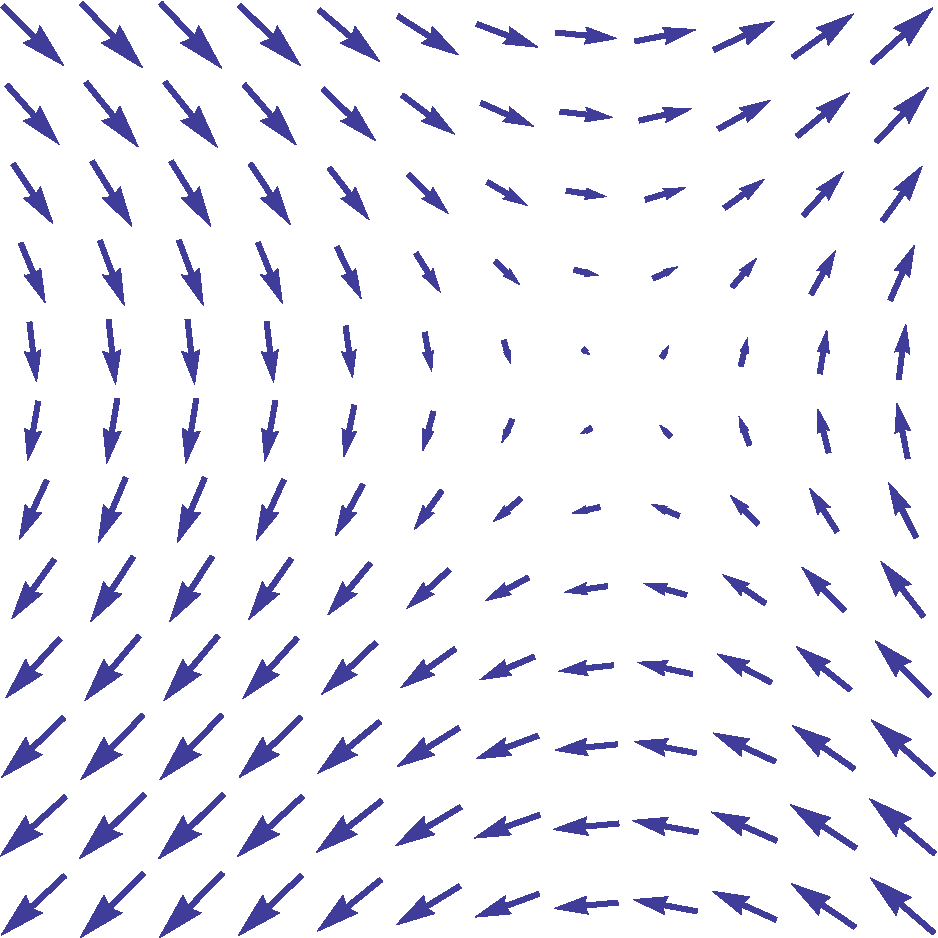
\includegraphics[width=0.5\textwidth]{figs/VectorField}

\hfill \tiny $\boldsymbol{\vec{\textbf{F}}} = \sin y \ih + \sin x \jh$
\end{minipage}

\vspace{-3mm}
\item the \emph{gradient} of a function $f(x,y)$:
    $$\grad f(x,y) = \frac{\partial f}{\partial x} \ih + \frac{\partial f}{\partial y} \jh$$

    \vspace{-2mm}
    \begin{itemize}
    \item the gradient \emph{is} a vector field:  $a=\frac{\partial f}{\partial x}$, $b=\frac{\partial f}{\partial y}$
    \item the gradient points uphill on the surface $z=f(x,y)$
    \end{itemize}
\item the \emph{differential} of $f$ contains the same information as the gradient: $df = \frac{\partial f}{\partial x}\,dx + \frac{\partial f}{\partial y}\,dy$
\end{enumerate}
\end{frame}


\begin{frame}{a major idea}

\begin{itemize}
\item \emph{some vector fields are gradients and some are not:}

\medskip
    \begin{itemize}
    \item Example which \emph{is} a gradient:
        $$\vF=\cos(x+y)\ih + (y+\cos(x+y))\jh$$
        $$\text{supply an $f$:} \hspace{4.0in}$$
        % f(x,y) = \frac{1}{2} y^2 + \sin(x+y)

\medskip
    \item Example which is \emph{not} a gradient:
        $$\vF=\cos(x+y)\ih + (x+\cos(x+y))\jh$$
        $$\text{explain why: \hspace{1.0in} \dots ?} \hspace{2.0in}$$
        % dM/dy = -\sin(x+y),  dN/dx = 1 - \sin(x+y)
    \end{itemize}
\item \emph{same idea}: some forms
    $$M(x,y)\,dx + N(x,y)\,dy$$
are the differentials of an $f$---they're \alert{exact}---and some are not
\item these ideas are \emph{not obvious}, but true!
\end{itemize}
\end{frame}


\begin{frame}{recall differentials}

\begin{itemize}
\item \emph{differentials} were introduced in first-semester calculus as a style for linearizations: $df = f'(x)\,dx$
\item now we need differentials for functions of 2 variables:
    $$f=f(x,y) \qquad \implies \qquad df = \frac{\partial f}{\partial x}\,dx + \frac{\partial f}{\partial y}\,dy$$

\vspace{-2mm}
    \begin{itemize}
    \item see calculus III
    \item differential of $f(x,y)$ describes the tangent plane to the surface $z=f(x,y)$
    \item the differential contains the same information as the gradient
    \item \alert{note:} you need to be able to compute partial derivatives!
    \end{itemize}
\item Example: find the differential of $f(x,y)=\frac{1}{2} y^2 + \sin(x+y)$

\vspace{20mm}
\end{itemize}
\end{frame}


\begin{frame}{how this relates to DEs}

\begin{itemize}
\item \emph{definition:}  a differential form
    $$M(x,y)\,dx + N(x,y)\,dy$$
is \alert{\emph{exact}} if there is $f(x,y)$ so that the form is a differential:
    $$M = \frac{\partial f}{\partial x}, \qquad N = \frac{\partial f}{\partial y}$$
\item \alert{main idea:} if we can rewrite an ODE as an exact differential form then we can solve the ODE
\end{itemize}
\end{frame}


\begin{frame}{example 1}

\begin{columns}
\begin{column}{0.65\textwidth}
\begin{itemize}
\item my first example uses a ``miracle'' at one step (\dots not sustainable!)
\item Example 1: solve
    $$y' = \frac{2y}{3y-2x}$$

\vspace{40mm}
\end{itemize}
\end{column}
\begin{column}{0.35\textwidth}
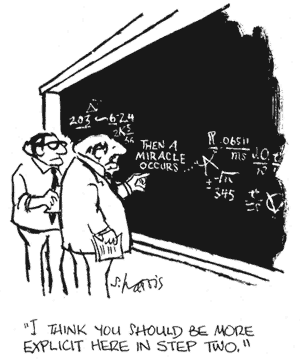
\includegraphics[width=\textwidth]{figs/miracle}

\vspace{20mm}
\end{column}
\end{columns}
\end{frame}


\begin{frame}{how to tell if it is exact}

\begin{itemize}
\item two concerns with above ``method'':
    \begin{enumerate}
    \item the differential form has to be exact!  how do you tell?
    \item I guessed $f(x,y)$; this is bad---needed miracle
    \end{enumerate}
\item the following theorem addresses concern 1:
\begin{theorem}
The differential form $M(x,y)\,dx + N(x,y)\,dy$ is exact if and only if
    $$\frac{\partial M}{\partial y} \stackrel{\ast}{=} \frac{\partial N}{\partial x}$$
\end{theorem}
    \begin{itemize}
    \item $\ast$ must be true on simply-connected domain like a rectangle
    \item \emph{proof of one direction}: if $M\,dx + N\,dy$ is exact then [fill in]
    \end{itemize}

\vspace{20mm}
\end{itemize}
\end{frame}


\begin{frame}{example 2}

\begin{itemize}
\item Example 2: use the method of Example 1 to solve
    $$y' = \frac{2y}{3y-x^2}$$

\vspace{40mm}
\item \dots trick question? \emph{no}
\item not every ODE is solvable by the ``exact'' method in \S 2.4
\item there is easy test for whether this method will work
\end{itemize}
\end{frame}


\begin{frame}{example 3}

\begin{itemize}
\item Example 3: is the equation exact?  if so, solve it:
    $$(2xy^2-3)\,dx + (2x^2y+4)\,dy = 0$$
\end{itemize}

\vspace{60mm}
\end{frame}


\begin{frame}{example 4}

\begin{itemize}
\item solve the given initial value problem:
    $$(e^x+y)\,dx + (2+x+ye^y)\,dy = 0, \quad y(0)=1$$
\end{itemize}

\vspace{60mm}
\end{frame}


\begin{frame}{example 4, cont.}

\end{frame}


\begin{frame}{straight from the book}

\begin{itemize}
\item the above examples have been straight from the book
    \begin{itemize}
    \item example 3 was \#5 in \S 2.4
    \item example 4 was \#22 in \S 2.4
    \end{itemize}
\item expect problems like these on Quizzes and Exams

\bigskip \bigskip
\item the next example is \#46 in \S 2.4
    \begin{itemize}
    \item it is \emph{too much computation} for a Quiz or Exam
    \end{itemize}
\end{itemize}
\end{frame}


\begin{frame}{example 5}

\begin{itemize}
\item Example 5:  the differential equation
    $$\frac{2xy}{(x^2+y^2)^2}\,dx + \left(1 + \frac{y^2-x^2}{(x^2+y^2)^2}\right)\,dy = 0$$
describes a family of curves which are the ``streamlines'' of a fluid flowing around a circular cylinder

    \begin{itemize}
    \item[(a)] solve the differential equation
        \begin{itemize}
        \item[$\circ$] get a general, but \emph{implicit}, solution
        \end{itemize}
    \item[(b)] there is one value of $c$ giving an explicit solution; find that
    \item[(c)] plot solution curves for $c=0,\pm 0.2, \pm 0.4, \pm 0.6, \pm 0.8$ using a contour plotting tool
    \end{itemize}
\end{itemize}

\vspace{-2mm}
\hfill 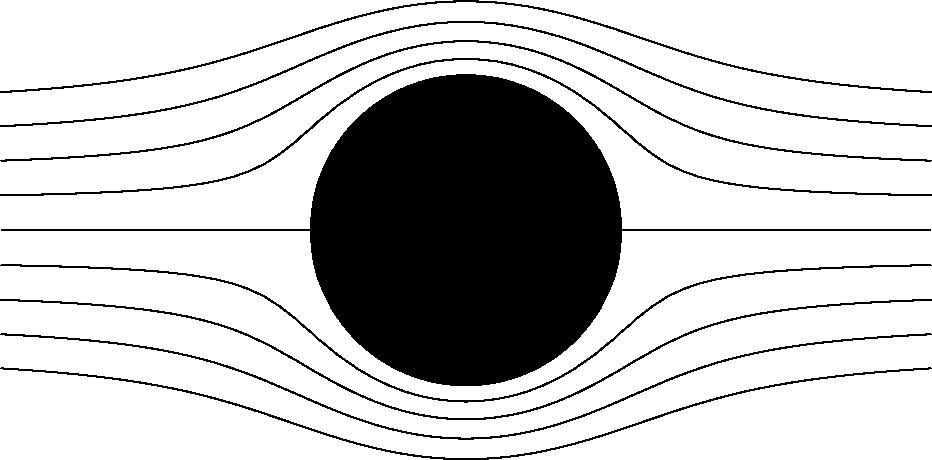
\includegraphics[width=0.45\textwidth]{figs/streamcyl-clean}
\end{frame}


\begin{frame}{example 5, cont.}

\begin{itemize}
\item X
\end{itemize}
\end{frame}


\begin{frame}{example 5, cont.$^2$}

\begin{itemize}
\item X
\end{itemize}
\end{frame}


\begin{frame}[fragile]
\frametitle{example 5, finished}

\begin{itemize}
\item Matlab/Octave code:
\begin{Verbatim}[fontsize=\footnotesize]
f = @(x,y) y.*(1.0 - 1.0./(x.^2+y.^2));    % define function
x = -3:.1:3;  [xx,yy] = meshgrid(x,x);     % grid of points
c = -0.8:0.2:0.8;                          % contours we want
h = contour(xx,yy,f(xx,yy),c,'k');         % black contours
clabel(h)                                  % ... with labels
axis equal                                 % looks better
\end{Verbatim}
\end{itemize}

\begin{center}
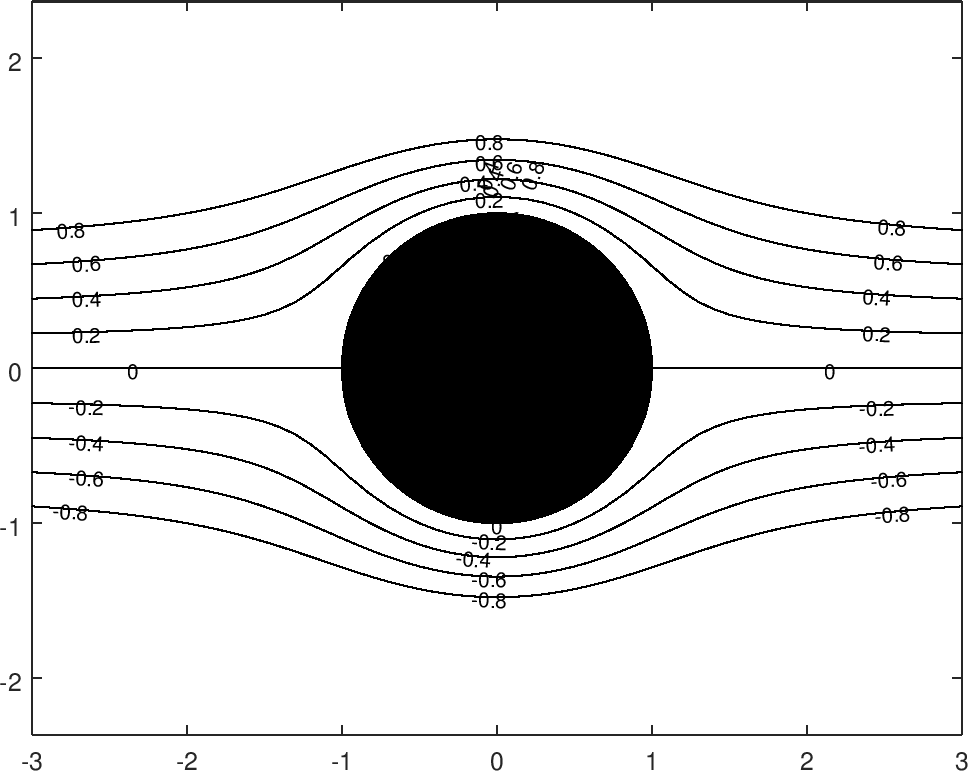
\includegraphics[width=0.5\textwidth]{figs/streamcyl-labeled}
\end{center}
\end{frame}


\begin{frame}{expectations}

to learn this material, just watching this video is \emph{not} enough; also
\begin{itemize}
\item \emph{watch} ``found online'' videos at

\centerline{\href{https://bueler.github.io/math302/week4.html}{\tt \color{cyan} bueler.github.io/math302/week4.html}}
%\item \emph{try-out} Euler's method codes at the same link
\item \emph{read} section 2.4 in the textbook
\item \emph{do} the WebAssign exercises for section 2.4
\end{itemize}

\bigskip
\alert{the biggest issue in \S 2.4 for most students:}

\centerline{partial derivatives, and integrals, are rusty}

\begin{itemize}
\item fix this now!
\item actually \emph{read} the relevant parts of a calculus book, starting with the first material on: (i) partial derivatives, (ii) vector fields, (iii) gradients, (iv) differentials
\item find a calc.~III student and try to help them learn these topics
\end{itemize}
\end{frame}

\end{document}

